\subsection{Alternative specifications for setting interest rates}
The monetary policy Taylor rule (\ref{tr}) sets the interest rate in response to contemporaneous output gap $y_t$ and inflation $\pi_t$. This contemporaneous rule assumes that the monetary authority observes current output gap and inflation.  Here we consider two alternative specifications for setting interest rates, widely used in the literature, and perhaps under more realistic informational assumptions of either forward-looking expectations (e.g. through survey data) or observing lagged variables.

\subsubsection{A forward-looking monetary policy rule}
As shown in Bullard and Mitra (2002) and Bullard et al. (2008),
another Taylor-type interest rate rule is to assume that the
monetary authorities set their interest rate instrument in response
to the forecasts of output and inflation deviations. This leads to
the forward expectations specification for the interest rate
equation, where (\ref{tr}) is replaced with
\begin{equation}\label{trexp}
     i_t=\phi_\pi\hat{E}_t\pi_{t+1}+\phi_y \hat{E}_ty_{t+1}.
\end{equation}
Thus the system (\ref{nkmodelm}) becomes
\begin{equation}\label{nkmodelmexp}
    \left\{
    \begin{split}
          {\bf x}_t&={\bf B}\hat{E}_t{\bf x}_{t+1}+{\bf C}\bf{u}_t,\\
          \bf{u}_t&={\pmb\rho}\bf{u}_{t-1}+\pmb{\varepsilon}_t,
    \end{split}
    \right.
\end{equation}
where ${\bf B}=\left[\begin{array}{cc}
1-\varphi\phi_y&\varphi(1-\phi_\pi)\\
\gamma(1-\varphi\phi_y)&\gamma\varphi(1-\phi_\pi)+\lambda
\end{array}\right],\,\,{\bf C}=\left[\begin{array}{cc} 1&0\\
\gamma&1
\end{array}\right].$

Similar to the above contemporaneous data interest rate rules, if the actual law of motion with the PLM in (\ref{xplm}) is stationary, the first-order autocorrelations (\ref{acynk}) and (\ref{acpink}) become\footnote{As in the baseline model above, the first -order sample autocorrelations of output gap and inflation computed based on time series simulationsl are consistent with the complicated expression for $G_{1}$ and $G_{2}$ in Eqs. (\ref{acynkexp}-\ref{acpinkexp}).}
\begin{eqnarray}
G_{1}(\beta_1,\beta_2) &=&\frac{\widetilde{f}_1}{\widetilde{g}_1}\label{acynkexp}\\
G_{2}(\beta_1,\beta_2)
&=&\frac{\widetilde{f}_2}{\widetilde{g}_2}\label{acpinkexp}
\end{eqnarray}
where
\begin{eqnarray*}
\widetilde{f}_1&=&\sigma_1^2\Big\{(\rho+\lambda_1+\lambda_2-\lambda\beta_2^2)[1-\lambda\beta_2^2(\rho+\lambda_1+\lambda_2)]+[\lambda\beta_2^2(\rho\lambda_1+\rho\lambda_2+\lambda_1\lambda_2)-\\
&&\rho\lambda_1\lambda_2][(\rho\lambda_1+\rho\lambda_2+\lambda_1\lambda_2)-\lambda\beta_2^2\rho\lambda_1\lambda_2]\Big\}+\sigma_2^2\Big\{(\varphi(1-\phi_\pi)\beta_2^2)^2[(\rho+\lambda_1+\lambda_2)\\
&&-\rho\lambda_1\lambda_2(\rho\lambda_1+\rho\lambda_2+\lambda_1\lambda_2)]\Big\},\\
\widetilde{g}_1&=&\sigma_1^2\Big\{[(1+\lambda^2\beta_2^4)-2\lambda\beta_2^2(\rho+\lambda_1+\lambda_2)+(1+\lambda^2\beta_2^4)(\rho\lambda_1+\rho\lambda_2+\lambda_1\lambda_2)]\\
&&-\rho\lambda_1\lambda_2[(1+\lambda^2\beta_2^4)(\rho+\lambda_1+\lambda_2)-2\lambda\beta_2^2(\rho\lambda_1+\rho\lambda_2+\lambda_1\lambda_2)+(1+\lambda^2\beta_2^4)\rho\lambda_1\lambda_2]\Big\}\\
&&+\sigma_2^2\Big\{(\varphi(1-\phi_\pi)\beta_2^2)^2[1+\rho\lambda_1+\rho\lambda_2+\lambda_1\lambda_2-\rho\lambda_1\lambda_2(\rho+\lambda_1+\lambda_2)-(\rho\lambda_1\lambda_2)^2]\Big\},\\
\end{eqnarray*}
\begin{eqnarray*}
\widetilde{f}_2&=&\sigma_1^2\Big\{\gamma^2[(\rho+\lambda_1+\lambda_2)-\rho\lambda_1\lambda_2(\rho\lambda_1+\rho\lambda_2+\lambda_1\lambda_2)]\Big\}+\sigma_2^2\Big\{[(\rho+\lambda_1+\lambda_2)-(1-\varphi\phi_y)\beta_1^2]\cdot\\
&&[1-(1-\varphi\phi_y)\beta_1^2(\rho+\lambda_1+\lambda_2)]+[(1-\varphi\phi_y)\beta_1^2(\rho\lambda_1+\rho\lambda_2+\lambda_1\lambda_2)-\rho\lambda_1\lambda_2]\cdot\\
&&[(\rho\lambda_1+\rho\lambda_2+\lambda_1\lambda_2)-(1-\varphi\phi_y)\beta_1^2\rho\lambda_1\lambda_2]\Big\},\\
\widetilde{g}_2&=&\sigma_1^2\Big\{\gamma^2[1+\rho\lambda_1+\rho\lambda_2+\lambda_1\lambda_2-\rho\lambda_1\lambda_2(\rho+\lambda_1+\lambda_2)-(\rho\lambda_1\lambda_2)^2]\Big\}\\
&&+\sigma_2^2\Big\{[1+((1-\varphi\phi_y)\beta_1^2)^2-2(1-\varphi\phi_y)\beta_1^2(\rho+\lambda_1+\lambda_2)+(1+((1-\varphi\phi_y)\beta_1^2)^2)\cdot\\
&&(\rho\lambda_1+\rho\lambda_2+\lambda_1\lambda_2)]-\rho\lambda_1\lambda_2[(1+((1-\varphi\phi_y)\beta_1^2)^2)(\rho+\lambda_1+\lambda_2)-2(1-\varphi\phi_y)\beta_1^2\cdot\\
&&(\rho\lambda_1+\rho\lambda_2+\lambda_1\lambda_2)+(1+((1-\varphi\phi_y)\beta_1^2)^2)\rho\lambda_1\lambda_2]\Big\},
\end{eqnarray*}
\begin{eqnarray*}
\lambda_1+\lambda_2&=&(1-\varphi\phi_y)\beta_1^2+(\gamma\varphi(1-\phi_\pi)+\lambda)\beta_2^2,\\
\lambda_1\lambda_2&=&\lambda(1-\varphi\phi_y)\beta_1^2\beta_2^2.
\end{eqnarray*}
In this case we have some similar results on the existence and stability as in the baseline model. Since the coefficients matrices are different, the corresponding sufficient conditions change.
\begin{cor}
\label{cor:exp} Under the forward-looking interest rate rule, if $\phi_y<\frac{1}{\varphi}$ and $1<\phi_\pi<1+\frac{\lambda}{\gamma\varphi}$, then there
exists at least one BLE $(\pmb\alpha^*,\pmb\beta^*)$, where
$\pmb\alpha^*=\bf 0=\overline{\bf x^*}$. Furthermore, the BLE $(\pmb\alpha^*,{\pmb\beta}^*)$ is locally
stable under SAC-learning if all the eigenvalues of $\pmb D\pmb G_{\pmb\beta}(\pmb\beta^*)=\Big(\frac{\partial G_i}{\partial \beta_j}\Big)_{{\pmb\beta}={\pmb\beta}^*}$ have real parts less than 1.
\end{cor}
\textbf{Proof.} See Appendix \ref{corfor}.

\begin{figure}
    \begin{center}
        \mbox{\subfigure[]
        {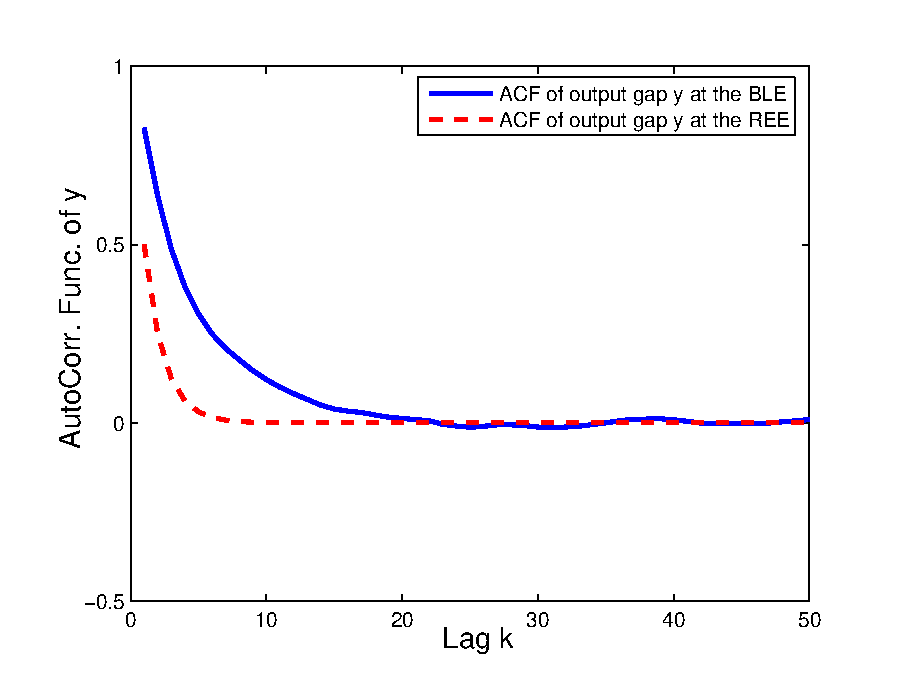
\includegraphics[width=3in]{acfytrexp2.eps}}\quad
        \subfigure[]
         {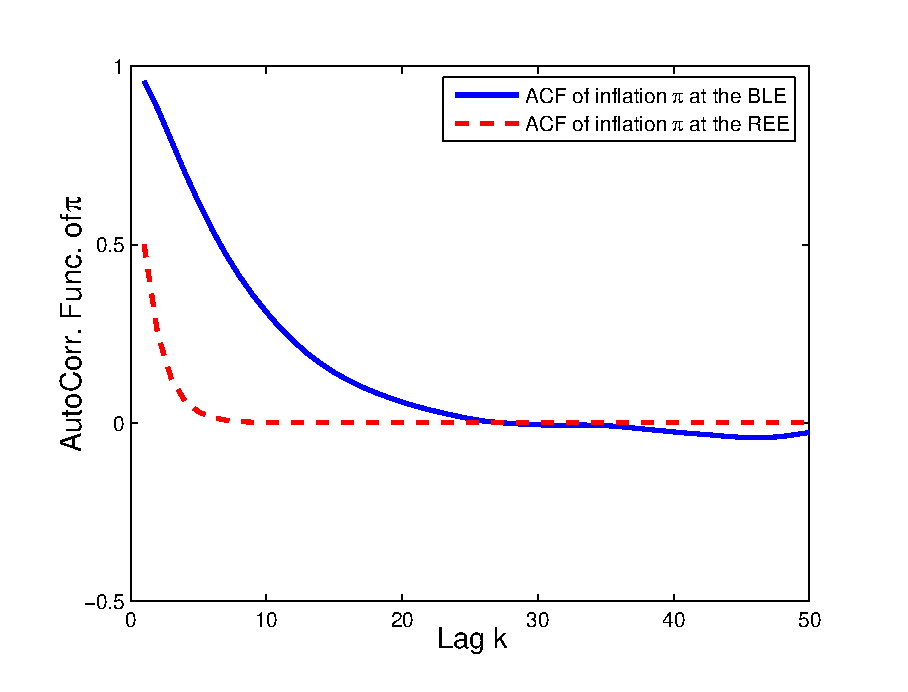
\includegraphics[width=3in]{acfpitrexp2.eps}}}
   \end{center}
   \caption{\label{aftrexp} Autocorrelation functions of output gap $y$ and inflation $\pi$ with forward-looking Taylor rule at the BLE $(\beta_1^*,
   \beta_2^*)=(0.8326, 0.9605)$. Parameters are: $\lambda=0.99, \varphi=1, \gamma=0.04, \rho=0.5, \phi_\pi=1.5,\phi_y=0.5, \sigma_{2}/\sigma_1=0.5$. }
    \end{figure}



\begin{figure}
    \begin{center}
        \mbox{\subfigure[]
        {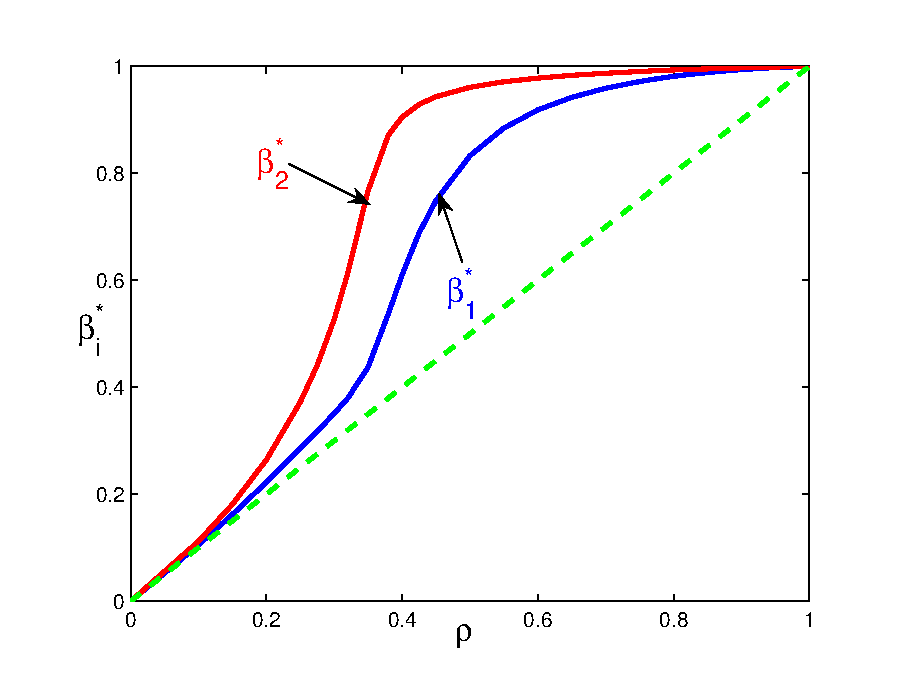
\includegraphics[width=3in]{blerhotrexp.eps}}
        \subfigure[]
         {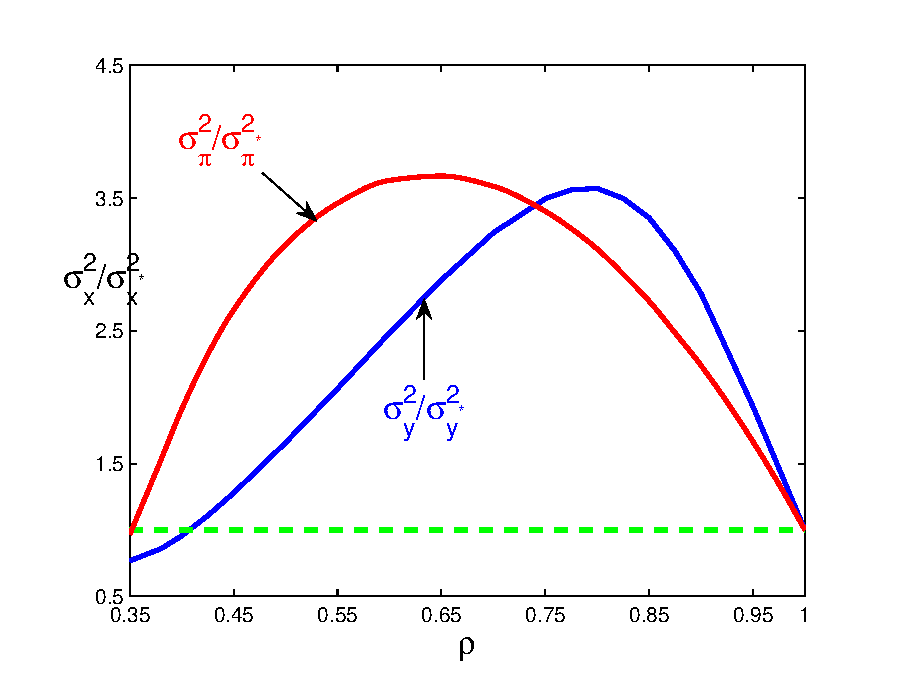
\includegraphics[width=3in]{varrhotrexp.eps}}}
   \end{center}
   \caption{ \label{blerhotrexp}
   BLE $(\beta^*_1, \beta^*_2)$ as a function of the persistence $\rho$ of the exogenous shocks with forward-looking Taylor rule (a) $\beta^*_i (i=1,2)$ with respect to $\rho$;  (b) the ratio of variances ($\sigma_y^2/\sigma_{y^*}^2$, $\sigma_\pi^2/\sigma_{\pi^*}^2$) with respect to $\rho$ at the corresponding BLE $(\beta^*_1, \beta^*_2)$. Parameters are: $\lambda=0.99, \varphi=1, \gamma=0.04, \phi_\pi=1.5,\phi_y=0.5, \frac{\sigma_2}{\sigma_1}=0.5$.  }
    \end{figure}

For the same benchmark parameter values as in the contemporaneous Taylor rule, the system has a BLE $(\beta_1^*,\beta_2^*)=(0.8326, 0.9605)$, with output and inflation much more persistent than the REE benchmark (with $\rho=0.5$), as illustrated in Figure \ref{aftrexp}. Figure \ref{blerhotrexp}a illustrates how these results depend on the parameter $\rho$, the persistence of the exogenous shocks. As before, for the forward looking Taylor rule, the system also displays {\it persistence amplification}, with the persistence of inflation and output gap along BLE much higher than the persistence $\rho$ of the exogenous shocks. Similarly, Figure \ref{blerhotrexp}b illustrates the excess volatility of inflation and output compared to the REE benchmark.

%Interestingly, we find multiple BLE here with proper parameters. For example, if we consider different parameters of $\phi_y$ and $\phi_\pi$ with $\phi_y=8$, $\phi_\pi=6$ and the other parameters given as in the benchmark case, we find three BLE $(\beta_1^*, \beta_2^*)=(0.9922,0.9664), (0.3203,0.8727), (-0.351, 0.8637)$, as shown in Figure \ref{BLEm_trexp}.

Here we also find finite optimal coefficients as for the contemporaneous Taylor rule. The difference is that here the optimal policy is $(\phi_y^*, \phi_\pi^*)=(1.1793,10.7942)$, which are both higher than in the contemporaneous case. We further study how the finite optimal coefficients respond as the persistence $\rho$ of shocks and the weight $\omega$ on inflation change. Figure \ref{optrhotrexp}a indicates that the finite optimal $\phi_\pi^*$ increases as $\rho$ varies around $0.5$, while $\phi_y^*$ changes only a little. This is because in this case the ratio $\sigma_\pi^2/\sigma_y^2$  of variances of inflation and output gap is relatively larger than in the contemporaneous case. For example, given the benchmark parameters, the variances of output gap and inflation at the BLE are $3.963$ and $4.097$ while they are $3.855$ and $3.595$, respectively, in the contemporaneous case. So here the variance of inflation plays a more important role and the finite optimal policy $\phi_\pi^*$ changes faster than $\phi_y^*$. Figure \ref{optomegatrexp} suggests similar effects of the weight of inflation $\omega$ on the finite optimal coefficients and optimal manifolds. Similar to the contemporaneous case, the optimal manifold moves up generally as $\rho$ or $\omega$ grows. In addition, Figure  \ref{optomegatrexp}b suggests that, as before, $\phi_\pi^*\approx 1.5$, if $\phi_y^*=0.5$ in the optimal manifold for $\omega=0.5$ in the framework of BLE and the loss function decreases very slowly till the finite optimal policy after $\phi_y^*=0.5$, as shown in Figure \ref{lossfopt_trexp}.

 \begin{figure}
    \begin{center}
       % \mbox{\subfigure[Effects of $\phi_{\pi}$ and $\phi_y$ on $\beta_1^*$]
%        {\includegraphics[width=3in]{blebeta1phipiC1.eps}}\quad
%        \subfigure[Effects of $\phi_{\pi}$ and $\phi_y$ on $\beta_2^*$]
%         {\includegraphics[width=3in]{blebeta2phipiC1.eps}}}
          \mbox{\subfigure[Optimal policy]
        {\includegraphics[width=3in]{optpolicyrho_trexp.eps}}\quad
        \subfigure[Optimal manifold]
         {\includegraphics[width=3in]{optmanifrho_trexp.eps}}}
        \end{center}
   \caption{ \label{optrhotrexp}
   Optimal policies at the BLE with respect to $\rho$ (a) and corresponding optimal manifolds for three different $\rho$ (connection points of solid and dotted curves corresponding to finite optimal policies) (b) with the forward-looking interest rate rule. Parameters are: $\lambda=0.99, \varphi=1, \gamma=0.04,\frac{\sigma_2}{\sigma_1}=0.5$ and $\omega=0.9$. }
    \end{figure}
    
    \begin{figure}
    \begin{center}
       % \mbox{\subfigure[Effects of $\phi_{\pi}$ and $\phi_y$ on $\beta_1^*$]
%        {\includegraphics[width=3in]{blebeta1phipiC1.eps}}\quad
%        \subfigure[Effects of $\phi_{\pi}$ and $\phi_y$ on $\beta_2^*$]
%         {\includegraphics[width=3in]{blebeta2phipiC1.eps}}}
          \mbox{\subfigure[Optimal policy]
        {\includegraphics[width=3in]{optpolicyomega_trexp.eps}}\quad
        \subfigure[Optimal manifold]
         {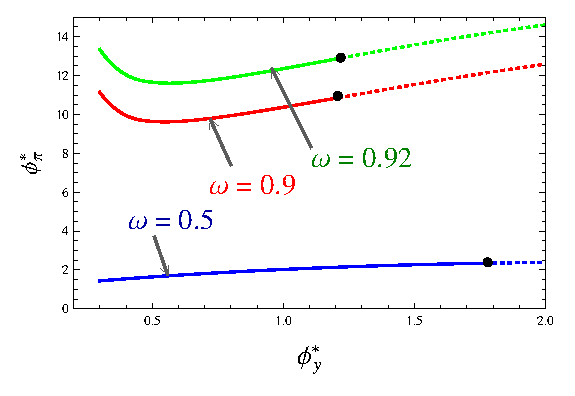
\includegraphics[width=3in]{optmanifomega_trexp.eps}}}
        \end{center}
   \caption{ \label{optomegatrexp}
  Optimal policies at the BLE with respect to $\omega$ (a) and corresponding optimal manifolds for three different $\omega$ (connection points of solid and dotted curves corresponding to finite optimal policies) (b) with the forward-looking interest rate rule.
   Parameters are: $\lambda=0.99, \varphi=1, \gamma=0.04, \sigma_{2}/\sigma_1=0.5$ and $\rho=0.5$. }
    \end{figure}
    
    \begin{figure}
    \begin{center}
        \mbox{\subfigure[]
        {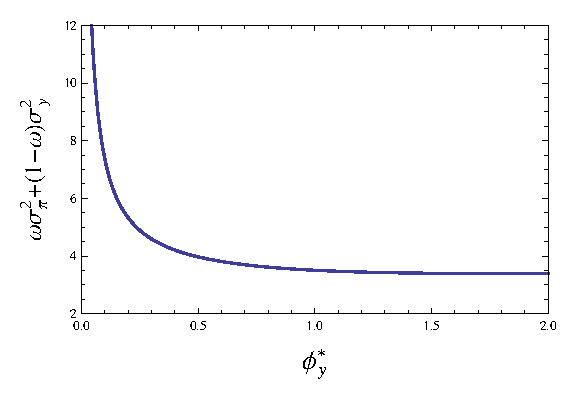
\includegraphics[width=3.2in]{optimalvar_trexp2.eps}}\quad
        \subfigure[]
         {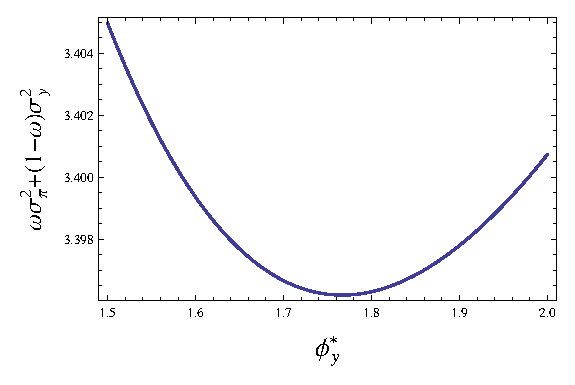
\includegraphics[width=3.2in]{optimalvar_trexp1.eps}}}
   \end{center}
   \caption{\label{lossfopt_trexp} Loss function along the optimal manifold in Figure \ref{optomegatrexp}(b) with $\omega=0.5$ for different ranges of $\phi_y^*$, i.e. $\phi_y^*\in [0, 2]$ (a) and  $\phi_y^*\in[1.5, 2]$ (b). Parameters are: $\lambda=0.99, \varphi=1, \gamma=0.04, \rho=0.5,
\frac{\sigma_2}{\sigma_1}=0.5$ and $\omega=0.5$.}
    \end{figure}
    
    \pagebreak

\subsubsection{A lagged monetary policy rule}
As argued e.g. in Bullard and Mitra (2002), it may be viewed as realistic for central bank practice to posit that the monetary authorities must react to last quarter's observations on
inflation and output gap as contemporaneous values are not known yet. This leads to the lagged data specification for the interest rate equation, where (\ref{tr}) is
replaced by
\begin{equation}\label{trlag}
     i_t=\phi_\pi\pi_{t-1}+\phi_y y_{t-1}.
\end{equation}
Due to the lagged monetary policy rule the system (\ref{nkmodelm}) includes an additional lagged term $x_{t-1}$ and becomes

\begin{equation}\label{nkmodelmlag}
    \left\{
    \begin{split}
          {\pmb x}_t&={\pmb A} {\pmb x}_{t-1}+{\pmb B} {\pmb x}_{t+1}^e+{\pmb C}\pmb{u}_t,\\
          \pmb{u}_t&={\pmb\rho}\pmb{u}_{t-1}+\pmb{\varepsilon}_t,
    \end{split}
    \right.
\end{equation}
where ${\pmb A}=\left[\begin{array}{cc}
-\varphi\phi_y&-\varphi\phi_\pi\\
-\gamma\varphi\phi_y&-\gamma\varphi\phi_\pi
\end{array}\right],\,\,{\pmb B}=\left[\begin{array}{cc}
1&\varphi\\
\gamma&\gamma\varphi+\lambda
\end{array}\right],\,\,{\pmb C}=\left[\begin{array}{cc} 1&0\\
\gamma&1
\end{array}\right].$

Similar to the above two interest rate rules, if the actual law of motion with the PLM in (\ref{xplm}) is stationary, %Besides the condition of existence and stability of BLE, the difference from the baseline model just lies in the expression of the first-order autocorrelations. In the case of the lagged rule, following similar calculations as in  the baseline model,
the first-order autocorrelations (\ref{acynk}) and (\ref{acpink})
become
%\footnote{As in the baseline line, the first-order autocorrelations of output gap and inflation calculated based on the time series generated by the model using the statistical definition of autocorrelation are consistent with those calculated based on the following equations. Hence although the expressions of $G_{1}$ and $G_{2}$ are extremely complicated, it can be sure that they are correct.}
\begin{eqnarray}
G_{1}(\beta_1,\beta_2) &=&\frac{\widetilde{f}_1}{\widetilde{g}_1}\label{acynklag}\\
G_{2}(\beta_1,\beta_2)
&=&\frac{\widetilde{f}_2}{\widetilde{g}_2}\label{acpinklag}
\end{eqnarray}
where
\begin{eqnarray*}
\widetilde{f}_1&=&\sigma_1^2\Big\{(\rho+\lambda_1+\lambda_2-\lambda\beta_2^2)[1-\lambda\beta_2^2(\rho+\lambda_1+\lambda_2)]+[\lambda\beta_2^2(\rho\lambda_1+\rho\lambda_2+\lambda_1\lambda_2)-\\
&&\rho\lambda_1\lambda_2][(\rho\lambda_1+\rho\lambda_2+\lambda_1\lambda_2)-\lambda\beta_2^2\rho\lambda_1\lambda_2]\Big\}+\sigma_2^2\Big\{(\varphi\phi_\pi-\varphi\beta_2^2)^2[(\rho+\lambda_1+\lambda_2)\\
&&-\rho\lambda_1\lambda_2(\rho\lambda_1+\rho\lambda_2+\lambda_1\lambda_2)]\Big\},\\
\widetilde{g}_1&=&\sigma_1^2\Big\{[(1+\lambda^2\beta_2^4)-2\lambda\beta_2^2(\rho+\lambda_1+\lambda_2)+(1+\lambda^2\beta_2^4)(\rho\lambda_1+\rho\lambda_2+\lambda_1\lambda_2)]\\
&&-\rho\lambda_1\lambda_2[(1+\lambda^2\beta_2^4)(\rho+\lambda_1+\lambda_2)-2\lambda\beta_2^2(\rho\lambda_1+\rho\lambda_2+\lambda_1\lambda_2)+(1+\lambda^2\beta_2^4)\rho\lambda_1\lambda_2]\Big\}\\
&&+\sigma_2^2\Big\{(\varphi\phi_\pi-\varphi\beta_2^2)^2[1+\rho\lambda_1+\rho\lambda_2+\lambda_1\lambda_2-\rho\lambda_1\lambda_2(\rho+\lambda_1+\lambda_2)-(\rho\lambda_1\lambda_2)^2]\Big\},\\
\end{eqnarray*}
\begin{eqnarray*}
\widetilde{f}_2&=&\sigma_1^2\Big\{\gamma^2[(\rho+\lambda_1+\lambda_2)-\rho\lambda_1\lambda_2(\rho\lambda_1+\rho\lambda_2+\lambda_1\lambda_2)]\Big\}+\sigma_2^2\Big\{[(\rho+\lambda_1+\lambda_2)-(\beta_1^2-\varphi\phi_y)]\cdot\\
&&[1-(\beta_1^2-\varphi\phi_y)(\rho+\lambda_1+\lambda_2)]+[(\beta_1^2-\varphi\phi_y)(\rho\lambda_1+\rho\lambda_2+\lambda_1\lambda_2)-\rho\lambda_1\lambda_2]\cdot\\
&&[(\rho\lambda_1+\rho\lambda_2+\lambda_1\lambda_2)-(\beta_1^2-\varphi\phi_y)\rho\lambda_1\lambda_2]\Big\},\\
\widetilde{g}_2&=&\sigma_1^2\Big\{\gamma^2[1+\rho\lambda_1+\rho\lambda_2+\lambda_1\lambda_2-\rho\lambda_1\lambda_2(\rho+\lambda_1+\lambda_2)-(\rho\lambda_1\lambda_2)^2]\Big\}\\
&&+\sigma_2^2\Big\{[(1+(\beta_1^2-\varphi\phi_y)^2)-2(\beta_1^2-\varphi\phi_y)(\rho+\lambda_1+\lambda_2)+(1+(\beta_1^2-\varphi\phi_y)^2)\cdot\\
&&(\rho\lambda_1+\rho\lambda_2+\lambda_1\lambda_2)]-\rho\lambda_1\lambda_2[(1+(\beta_1^2-\varphi\phi_y)^2)(\rho+\lambda_1+\lambda_2)-2(\beta_1^2-\varphi\phi_y)\cdot\\
&&(\rho\lambda_1+\rho\lambda_2+\lambda_1\lambda_2)+(1+(\beta_1^2-\varphi\phi_y)^2)\rho\lambda_1\lambda_2]\Big\},
\end{eqnarray*}
\begin{eqnarray*}
\lambda_1+\lambda_2&=&\beta_1^2-\varphi\phi_y-\gamma\varphi\phi_\pi+(\gamma\varphi+\lambda)\beta_2^2,\\
\lambda_1\lambda_2&=&\lambda(\beta_1^2-\varphi\phi_y)\beta_2^2.
\end{eqnarray*}

Note that, because of the additional lagged term $x_{t-1}$, the rational expectations equilibrium is different compared to the system without this lagged term ${\pmb x}_{t-1}$ in the previous two cases. The proofs concerning existence and stability of BLE, however, are straightforward extensions of the proofs without the additional term ${\pmb x}_{t-1}$\footnote{In particular, the system (\ref{nkmodelmlag}) can be rewritten in the form of Eq. (\ref{modeln30}) in appendix \ref{acfnkc}, when BLE is considered. The difference from the baseline case lies in different coefficient matrices $ {\bf z}_{t}=\pmb{(A+B\beta^2)}{\bf z}_{t-1}+\pmb{C\varepsilon}_t+\pmb{C\rho I \varepsilon}_{t-1}+\cdots$ with matrices ${\bf A, B, C}$ as in the system (\ref{nkmodelmlag}). Then following the same idea of the proof, the first-order autocorrelations for the lagged monetary policy rule in (\ref{acynklag}) and (\ref{acpinklag}) are obtained. Similar proofs of propositions 1 and 2, concerning existence and stability of BLE, can then be obtained.}. In this case we have similar results on the existence and stability on BLE as in the baseline model.
\begin{cor}
\label{cor:lag} Under the lagged interest rate rule, if $\phi_y<\frac{1}{\varphi}$ and $1<\phi_\pi<\frac{1-\varphi\phi_y}{\gamma\varphi}$, then there
exists at least one BLE $(\pmb\alpha^*,\pmb\beta^*)$. Furthermore, the BLE $(\pmb\alpha^*,{\pmb\beta}^*)$ is locally
stable under SAC-learning if all the eigenvalues of $\pmb D\pmb G_{\pmb\beta}(\pmb\beta^*)=\Big(\frac{\partial G_i}{\partial \beta_j}\Big)_{{\pmb\beta}={\pmb\beta}^*}$ have real parts less than 1.
\end{cor}
\textbf{Proof.} See Appendix \ref{corlagproof}.

\begin{figure}
    \begin{center}
        \mbox{\subfigure[ ]
        {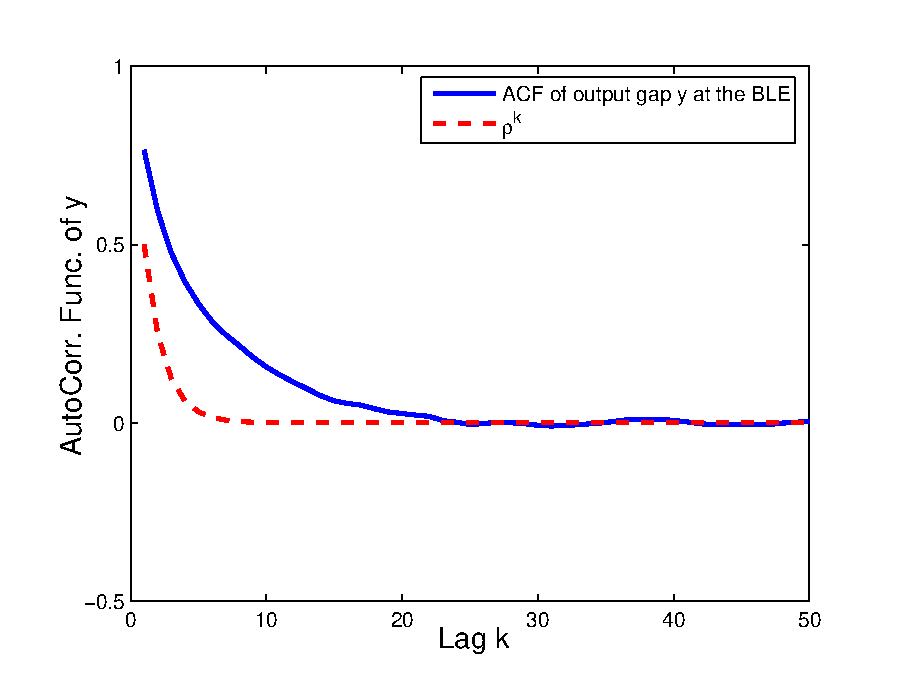
\includegraphics[width=3in]{acfytrlag2.eps}}\quad
        \subfigure[]
         {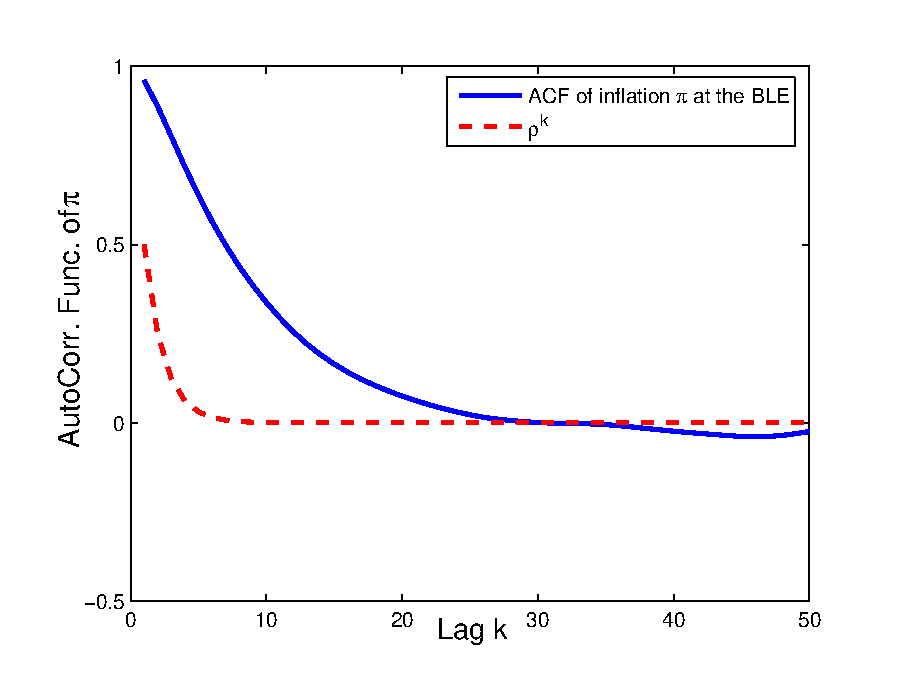
\includegraphics[width=3in]{acfpitrlag2.eps}}}
   \end{center}
   \caption{\label{aftrlag} Autocorrelation functions of output gap $y$ and inflation $\pi$ with lagged Taylor rule at the BLE $(\beta_1^*,
   \beta_2^*)=(0.7746, 0.9628)$. Parameters are: $\lambda=0.99, \varphi=1, \gamma=0.04, \rho=0.5, \phi_\pi=1.5,\phi_y=0.5, \sigma_{2}/\sigma_1=0.5$.}
    \end{figure}
    
    \begin{figure}
    \begin{center}
    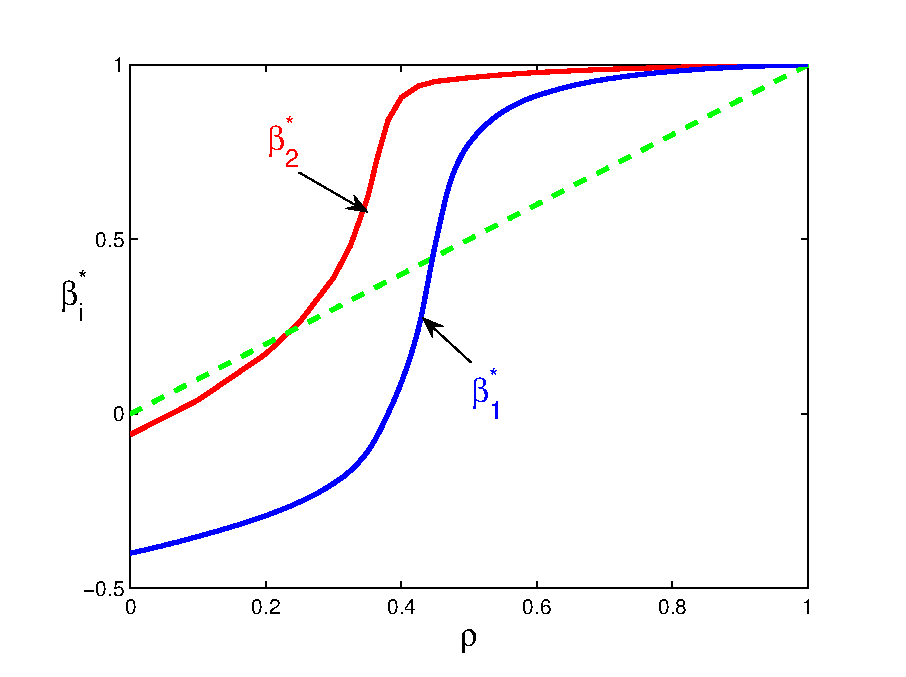
\includegraphics[width=4in]{blerhotrlag.eps}
       % %\mbox{\subfigure[]
%        {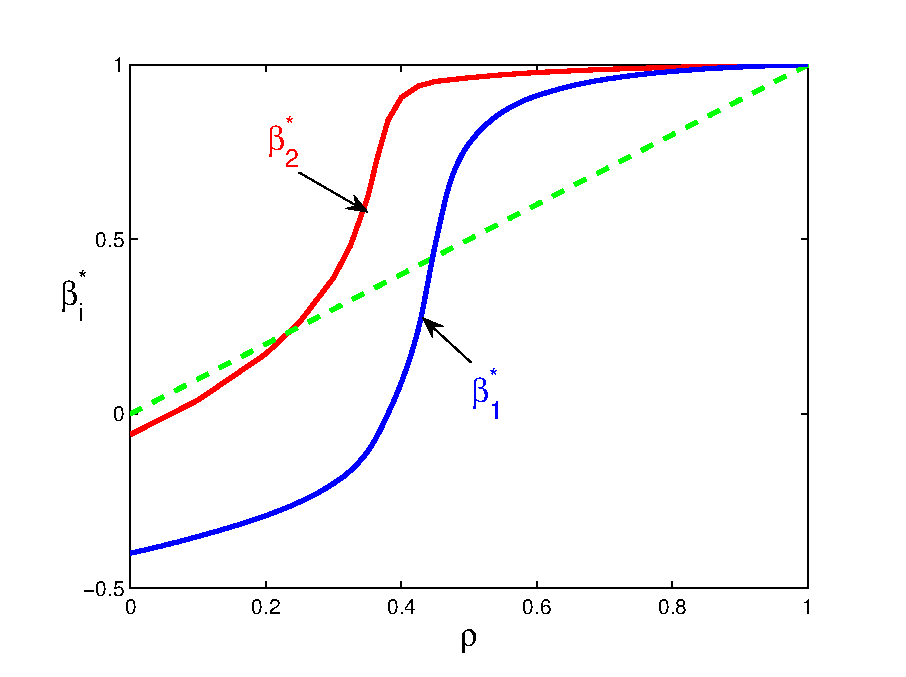
\includegraphics[width=3in]{blerhotrlag.eps}}\quad
%        %\subfigure[]
%%         {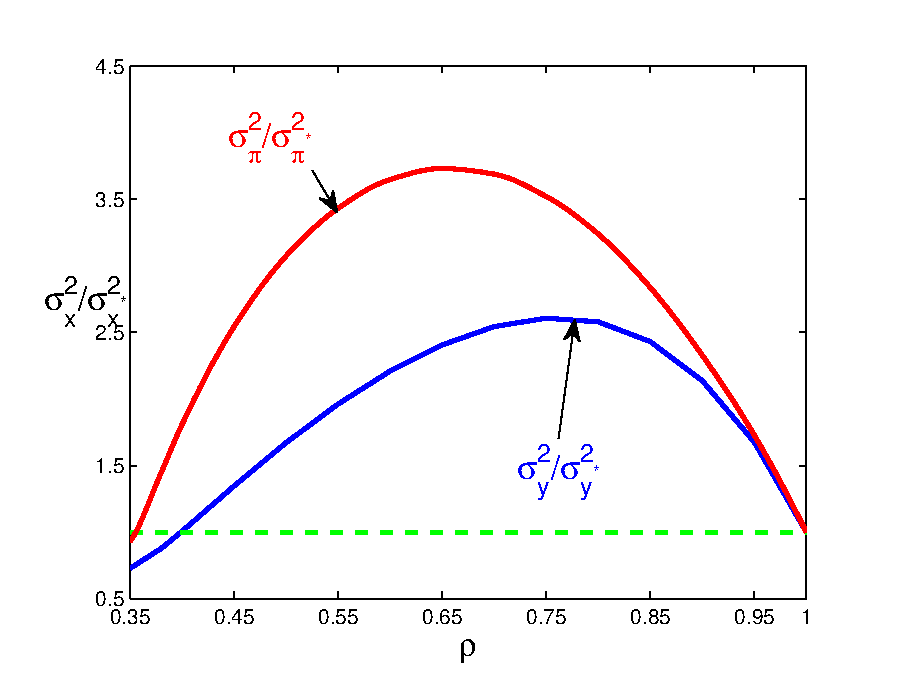
\includegraphics[width=3in]{varrhotrc.eps}}
%}
   \end{center}
   \caption{ \label{blerhotrlag} Effects of $\rho$ with lagged Taylor rule, i.e. $\beta^*_i (i=1,2)$ with respect to $\rho$. Parameters are: $\lambda=0.99, \varphi=1, \gamma=0.04, \phi_\pi=1.5,\phi_y=0.5, \frac{\sigma_2}{\sigma_1}=0.5$. }
    \end{figure}

For the same benchmark parameter values as before, the system has a BLE $(\beta_1^*,\beta_2^*)=(0.7746, 0.9628)$. Figure \ref{aftrlag} illustrates the ACF of output and inflation along the BLE and shows that they are much more persistent than the autocorrelations in the exogenous shocks. Figure \ref{blerhotrlag} illustrates that the model with a lagged Taylor rule also exhibits {\it persistence amplification} within the empirically relevant region of parameters $\rho\geq 0.5$ (cf. footnote\ref{note:emprel}).
% Interestingly, we find multiple BLE here with proper parameters. For example, if we consider different parameters of $\phi_y$ and $\phi_\pi$ with $\phi_y=0.8$, $\phi_\pi=1.85$ and the other parameters given as in the benchmark case, we find three BLE $(\beta_1^*, \beta_2^*)=(0.5848, 0.9626), (0.3992,0.9659), (0.1182,0.9678)$, as shown in Figure \ref{BLEm_trlag}.


Here we find finite optimal coefficients again as in the contemporaneous and forward-looking Taylor rules. The difference is that here the optimal policy is $(\phi_y^*, \phi_\pi^*)=(0.4566, 5.2008)$. We further study how the finite optimal coefficients respond as the persistence $\rho$ of shocks and the weight on inflation $\omega$ change. Figure \ref{optrhotrlag}a indicates that finite optimal $\phi_\pi^*$ increases as $\rho$ varies around $0.5$ while $\phi_y^*$ changes just a little, similar to the forward-looking case. This is also because in this case the ratio of variances of inflation and output gap is also larger than in the contemporaneous case, that is, the variance of inflation plays a more dominant role.  For example, given the benchmark parameters, the variances of output gap and inflation at the BLE are $3.145$ and $4.310$, while they are $3.855$ and $3.595$, respectively, in the contemporaneous case. Therefore, similar to the forward-looking case, the finite optimal policy $\phi_\pi^*$  changes faster than $\phi_y^*$. Figure \ref{optomegatrlag} suggests similar effects of the weight on inflation $\omega$ on the finite optimal coefficients and optimal manifolds. In addition, if we consider $\omega=0.5$, Figure \ref{lossfopt_trlag} suggests that, as before, $(\phi_y^*,\phi_\pi^*)=(0.5, 1.5)$ is nearly optimal in the case the weight $\omega=0.5$.

\begin{figure}
    \begin{center}
       % \mbox{\subfigure[Effects of $\phi_{\pi}$ and $\phi_y$ on $\beta_1^*$]
%        {\includegraphics[width=3in]{blebeta1phipiC1.eps}}\quad
%        \subfigure[Effects of $\phi_{\pi}$ and $\phi_y$ on $\beta_2^*$]
%         {\includegraphics[width=3in]{blebeta2phipiC1.eps}}}
          \mbox{\subfigure[Optimal policy]
        {\includegraphics[width=3in]{optpolicyrho_trlag.eps}}\quad
        \subfigure[Optimal manifold]
         {\includegraphics[width=3in]{optmanifrho_trlag.eps}}}
        \end{center}
   \caption{ \label{optrhotrlag}
  Optimal policies at the BLE with respect to $\rho$ (a) and corresponding optimal manifolds for three different $\rho$ (connection points of solid and dotted curves corresponding to finite optimal policies) (b) with the lagged interest rate rule.
   Parameters are: $\lambda=0.99, \varphi=1, \gamma=0.04, \sigma_{2}/\sigma_1=0.5$ and $\omega=0.9$. }
    \end{figure}
    
\begin{figure}
    \begin{center}
       % \mbox{\subfigure[Effects of $\phi_{\pi}$ and $\phi_y$ on $\beta_1^*$]
%        {\includegraphics[width=3in]{blebeta1phipiC1.eps}}\quad
%        \subfigure[Effects of $\phi_{\pi}$ and $\phi_y$ on $\beta_2^*$]
%         {\includegraphics[width=3in]{blebeta2phipiC1.eps}}}
          \mbox{\subfigure[Optimal policy]
        {\includegraphics[width=3in]{optpolicyomega_trlag.eps}}\quad
        \subfigure[Optimal manifold]
         {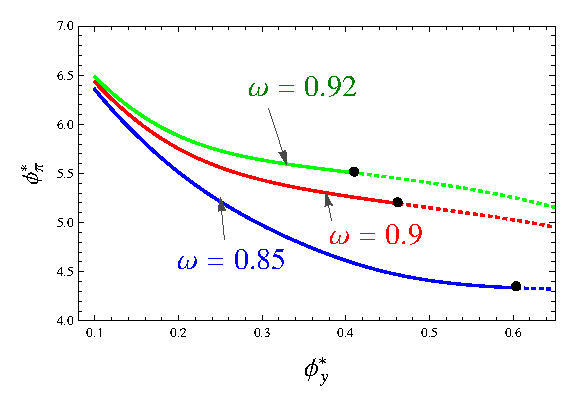
\includegraphics[width=3in]{optmanifomega_trlag.eps}}}
        \end{center}
   \caption{ \label{optomegatrlag}
  Optimal policies at the BLE with respect to $\omega$ (a) and corresponding optimal manifolds for three different $\omega$ (connection points of solid and dotted curves corresponding to finite optimal policies) (b) with the lagged interest rate rule.
   Parameters are: $\lambda=0.99, \varphi=1, \gamma=0.04,\sigma_{2}/\sigma_1=0.5$ and $\rho=0.5$. }
    \end{figure}    
    
 \begin{figure}
    \begin{center}
        \mbox{\subfigure[Optimal manifold]
        {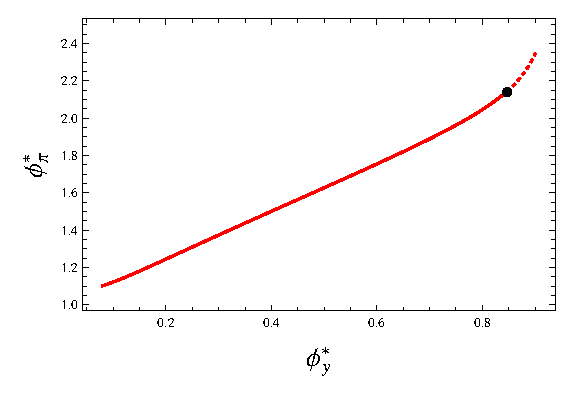
\includegraphics[width=3in]{optmanifomega05_trlag.eps}}\quad
        \subfigure[Loss function]
         {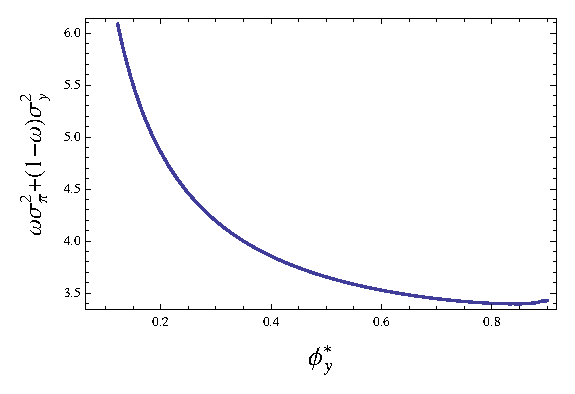
\includegraphics[width=3in]{varoptpolicyomega05_trlag.eps}}}
        \end{center}
   \caption{ \label{lossfopt_trlag}
  Optimal manifold at the BLE for $\omega=0.5$ (connection points of solid and dotted curves corresponding to finite optimal policies) (a) and corresponding loss function along the optimal manifold(b) with the lagged interest rate rule.
   Parameters are: $\lambda=0.99, \varphi=1, \gamma=0.04, \rho=0.5, \sigma_{2}/\sigma_1=0.5$, $\omega=0.5$. }
    \end{figure}   